\documentclass[journal,12pt,twocolumn]{IEEEtran}
%
\usepackage{setspace}
\usepackage{gensymb}
\usepackage{xcolor}
\usepackage{caption}
%\usepackage{subcaption}
%\doublespacing
\singlespacing
\usepackage{multicol}

\usepackage{iithtlc}
%\usepackage{graphicx}
%\usepackage{amssymb}
%\usepackage{relsize}
\usepackage[cmex10]{amsmath}
\usepackage{mathtools}
%\usepackage{amsthm}
%\interdisplaylinepenalty=2500
%\savesymbol{iint}
%\usepackage{txfonts}
%\restoresymbol{TXF}{iint}
%\usepackage{wasysym}
\usepackage{amsthm}
\usepackage{mathrsfs}
\usepackage{txfonts}
\usepackage{stfloats}
\usepackage{cite}
\usepackage{cases}
\usepackage{subfig}
%\usepackage{xtab}
\usepackage{longtable}
\usepackage{multirow}
%\usepackage{algorithm}
%\usepackage{algpseudocode}
\usepackage{enumitem}
\usepackage{mathtools}
%\usepackage{stmaryrd}
\usepackage{graphicx}
\usepackage{listings}
    \usepackage[latin1]{inputenc}                                 %%
    \usepackage{color}                                            %%
    \usepackage{array}                                            %%
    \usepackage{longtable}                                        %%
    \usepackage{calc}                                             %%
    \usepackage{multirow}                                         %%
    \usepackage{hhline}                                           %%
    \usepackage{ifthen}                                           %%
  %optionally (for landscape tables embedded in another document): %%
    \usepackage{lscape}     
\usepackage{url}
\def\UrlBreaks{\do\/\do-}

%\usepackage{wasysym}
%\newcounter{MYtempeqncnt}
\DeclareMathOperator*{\Res}{Res}
%\renewcommand{\baselinestretch}{2}
\renewcommand\thesection{\arabic{section}}
\renewcommand\thesubsection{\thesection.\arabic{subsection}}
\renewcommand\thesubsubsection{\thesubsection.\arabic{subsubsection}}

\renewcommand\thesectiondis{\arabic{section}}
\renewcommand\thesubsectiondis{\thesectiondis.\arabic{subsection}}
\renewcommand\thesubsubsectiondis{\thesubsectiondis.\arabic{subsubsection}}

% correct bad hyphenation here
\hyphenation{op-tical net-works semi-conduc-tor}

\def\inputGnumericTable{}  

\lstset{
language=python,
frame=single, 
breaklines=true
}

\begin{document}
%

\theoremstyle{definition}

\newtheorem{theorem}{Theorem}[section]
\newtheorem{problem}{Problem}
\newtheorem{proposition}{Proposition}[section]
\newtheorem{lemma}{Lemma}[section]
\newtheorem{corollary}[theorem]{Corollary}
\newtheorem{example}{Example}[section]
\newtheorem{definition}{Definition}[section]
%\newtheorem{algorithm}{Algorithm}[section]
%\newtheorem{cor}{Corollary}
\newcommand{\BEQA}{\begin{eqnarray}}
\newcommand{\EEQA}{\end{eqnarray}}
\newcommand{\define}{\stackrel{\triangle}{=}}

\bibliographystyle{IEEEtran}
%\bibliographystyle{ieeetr}



\providecommand{\pr}[1]{\ensuremath{\Pr\left(#1\right)}}
\providecommand{\qfunc}[1]{\ensuremath{Q\left(#1\right)}}
\providecommand{\sbrak}[1]{\ensuremath{{}\left[#1\right]}}
\providecommand{\lsbrak}[1]{\ensuremath{{}\left[#1\right.}}
\providecommand{\rsbrak}[1]{\ensuremath{{}\left.#1\right]}}
\providecommand{\brak}[1]{\ensuremath{\left(#1\right)}}
\providecommand{\lbrak}[1]{\ensuremath{\left(#1\right.}}
\providecommand{\rbrak}[1]{\ensuremath{\left.#1\right)}}
\providecommand{\cbrak}[1]{\ensuremath{\left\{#1\right\}}}
\providecommand{\lcbrak}[1]{\ensuremath{\left\{#1\right.}}
\providecommand{\rcbrak}[1]{\ensuremath{\left.#1\right\}}}
\theoremstyle{remark}
\newtheorem{rem}{Remark}
\newcommand{\sgn}{\mathop{\mathrm{sgn}}}
\providecommand{\abs}[1]{\left\vert#1\right\vert}
\providecommand{\res}[1]{\Res\displaylimits_{#1}} 
\providecommand{\norm}[1]{\lVert#1\rVert}
\providecommand{\mtx}[1]{\mathbf{#1}}
\providecommand{\mean}[1]{E\left[ #1 \right]}
\providecommand{\fourier}{\overset{\mathcal{F}}{ \rightleftharpoons}}
%\providecommand{\hilbert}{\overset{\mathcal{H}}{ \rightleftharpoons}}
\providecommand{\system}{\overset{\mathcal{H}}{ \longleftrightarrow}}
\providecommand{\gauss}[2]{\mathcal{N}\ensuremath{\left(#1,#2\right)}}
	%\newcommand{\solution}[2]{\textbf{Solution:}{#1}}
\newcommand{\solution}{\noindent \textbf{Solution: }}
\providecommand{\dec}[2]{\ensuremath{\overset{#1}{\underset{#2}{\gtrless}}}}
%\numberwithin{equation}{section}
%\numberwithin{problem}{section}

\def\putbox#1#2#3{\makebox[0in][l]{\makebox[#1][l]{}\raisebox{\baselineskip}[0in][0in]{\raisebox{#2}[0in][0in]{#3}}}}
     \def\rightbox#1{\makebox[0in][r]{#1}}
     \def\centbox#1{\makebox[0in]{#1}}
     \def\topbox#1{\raisebox{-\baselineskip}[0in][0in]{#1}}
     \def\midbox#1{\raisebox{-0.5\baselineskip}[0in][0in]{#1}}


% paper title
% can use linebreaks \\ within to get better formatting as desired

\title{\logo{FM Signal Reception using Pi}}
 
%
%
% author names and IEEE memberships
% note positions of commas and nonbreaking spaces ( ~ ) LaTeX will not break
% a structure at a ~ so this keeps an author's name from being broken across
% two lines.
% use \thanks{} to gain access to the first footnote area
% a separate \thanks must be used for each paragraph as LaTeX2e's \thanks
% was not built to handle multiple paragraphs
%

%\author{Y Aditya, A Rathnakar and G V V Sharma$^{*}$% <-this % stops a space
\author{K Prasanna Kumar and G V V Sharma %<-this  stops a space
\thanks{The authors are with the Department
of Electrical Engineering, IIT, Hyderabad
502285 India $1^{st}$ e-mail:  kk.prassu924@gmail.com  $2^nd$ e-mail: \{gadepall\}@iith.ac.in. 
}}



% make the title area
\maketitle


\tableofcontents
\bigskip
\begin{abstract}
This module explains how to interface RTL-SDR dongle with Raspbery Pi and Demodulate FM Signal.
\end{abstract}
\section{Software Installation}
\subsection{Preliminary Tools }
If you do not have GIT, cmake \& unzip installed them using following commands.
\begin{lstlisting}[frame = single]
 sudo apt-get update
 sudo apt-get install git-core
 sudo apt-get install cmake
 sudo apt-get install unzip
\end{lstlisting}
\subsection{Update \& Install Dependencies}
Update the internal repository of Pi
\begin{lstlisting}{frame = single}
sudo apt-get update
\end{lstlisting}

Download or clone dependencies.html file from the github to know list of dependencies required to interface RTL-SDR dongle.
\begin{lstlisting}{frame = single}
git clone https://github.com/PrasannaIITH/UHD-dependencies.git
cd UHD-dependencies
unzip dependencies.zip
\end{lstlisting}

Open the .html page in the directory using browser 
\begin{lstlisting}{frame = single}
ls
chromium-browser ./Dependencies.html
\end{lstlisting}

Open a new terminal and install the dependencies which are present in the page as per instructions.
\subsection{Download \& Build RTL-SDR software}
Download or clone from github:
\begin{lstlisting}{frame = single}
git clone git://git.osmocom.org/rtl-sdr.git
          (or)
git clone https://github.com/PrasannaIITH/rtl-sdr.git
\end{lstlisting}
Build with cmake :
\begin{lstlisting}{frame = single}
cd rtl-sdr
mkdir build
cd build
cmake ../
make 
sudo make install
sudo ldconfig 
\end{lstlisting}

In order to be able to use the dongle as a non-root user, you may install the appropriate udev rules file by calling cmake with the following command in build directory. 
\begin{lstlisting}{frame = single}
cmake ../ -DINSTALL_UDEV_RULES=ON
\end{lstlisting}

Building with auto tools: 
\begin{lstlisting}{frame = single}
cd
cd rtl-sdr/
autoreconf -i
./configure
make
sudo make install
sudo ldconfig
\end{lstlisting}

In order to be able to use the dongle as a non-root user, you may install the appropriate udev rules file by calling
\begin{lstlisting}{frame = single}
cd
cd rtl-sdr/
sudo make install-udev-rules
\end{lstlisting}

we can see \textit{rtl\_ tcp, rtl\_ test \& rtl\_ sdr} in \textit{rtl-sdr/src} directory. By this we can say the software is  successfully.
\section{Hardware Installation}
We use DVB-T RTL-SDR R820TU dongle with antenna as RF front-end. 
\begin{figure}[h!]
\centering
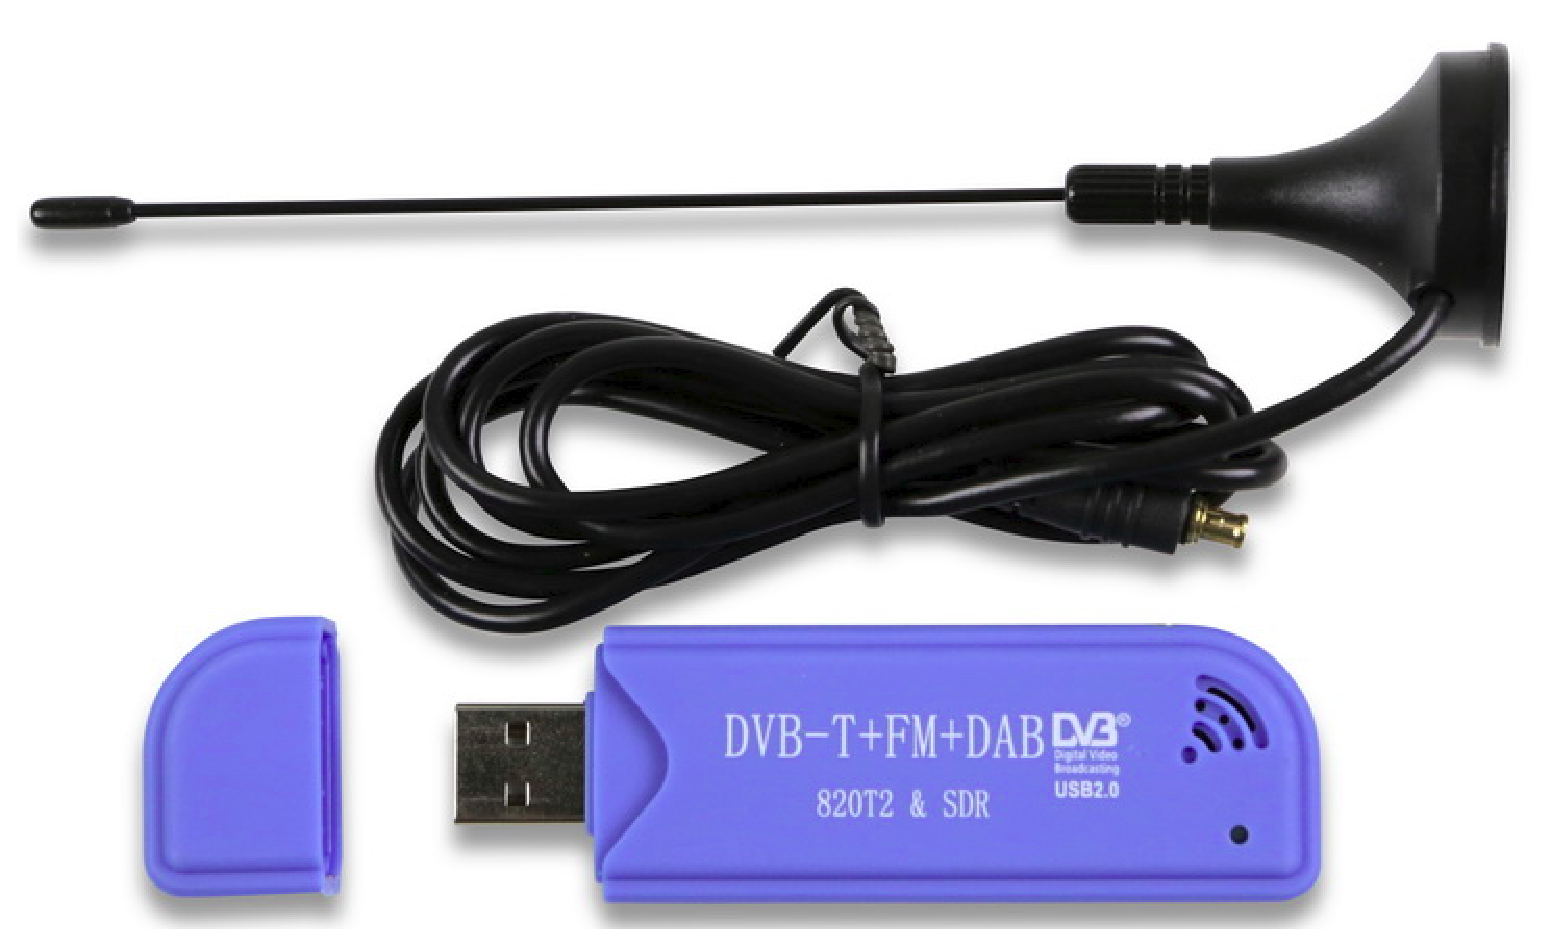
\includegraphics[scale=0.28]{Figures/rtlsdr_dongle}
\caption{DVB -T RTL-SDR Dongle}
\end{figure}
\subsection{Interior Components}
\begin{figure}[h!]
\centering
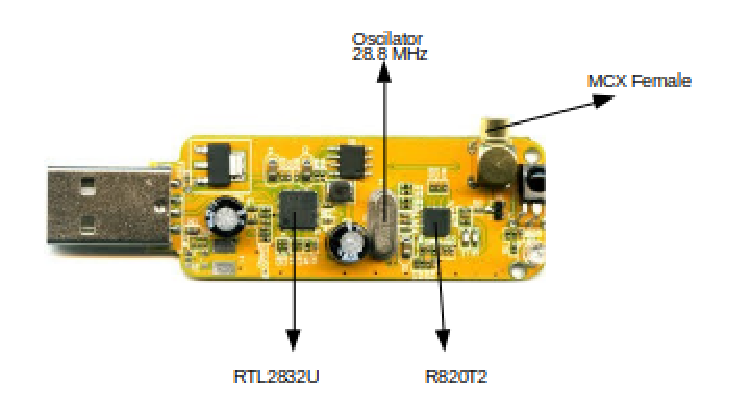
\includegraphics[scale=0.8]{Figures/inner_dia}
\caption{Components of RTL-SDR Dongle}
\end{figure}
\subsection{Working Process}
RTL-SDR Dongle consists of two important blocks \textbf{Radio tuner} \& \textbf{Demodulator with ADC}.
\begin{figure}[h!]
\centering
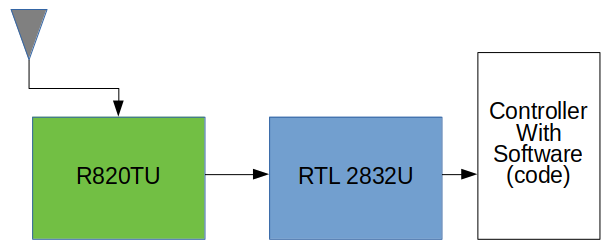
\includegraphics[scale=0.32]{Figures/RTL-ARC}
\caption{Block Diagram}
\end{figure}
\begin{enumerate}
\item \textbf{Antenna:} Antenna converts the electromagnetic signal to electrical analog signal.
\item \textbf{Radio Tuner:} R820T2 chip is an radio tuner here, it converts high frequency signal to a lower intermediate frequency.
\item \textbf{Demodulator:}  RTL2832U helps to demodulate the signal and convert the analog signal to digital. 
\item The digital signal with help of USB fed to the computer. 
\end{enumerate}
\subsection{Test Connection}
Connect the dongle to Pi, connect the antenna to the dongle with help of MCX Male \& Female.  Now run the following command in the terminal to see device details.
\begin{lstlisting}{frame = single}
rtl_tcp
\end{lstlisting}
\section{Operation}
Run the following commands to receive \& play audio single from the FM transmitter
\begin{lstlisting}{frame = single}
cd rtl-sdr
cd src
sudo ./rtl_fm -f 89.9e6 -M wbfm -s 200000 -r 48000 - | aplay -r 48k -f S16_LE
\end{lstlisting}

\begin{thebibliography}{00}
\bibitem{b1} Open Source Mobile Communications, \url{https://osmocom.org/}. 
\bibitem{b2} RTL-SDR Dongle and GQRX on Mac  \url{https://www.youtube.com/watch?v=bSAa2aOXpCc}.
\bibitem{b3} Official Osmocom mirror, Mirror of the git.osmocom.org repositories \url{https://github.com/osmocom}.
\end{thebibliography}
\end{document}